\documentclass[10pt,a4paper]{article}
\usepackage[latin1]{inputenc}
\usepackage{amsmath}
\usepackage{microtype}
\usepackage[none]{hyphenat}
\usepackage{verbatim}
\usepackage{amsfonts}
\usepackage{amssymb}
\usepackage{enumitem}
\renewcommand{\familydefault}{\sfdefault}
\usepackage{mathpazo}
\renewcommand{\rmdefault}{put}
\usepackage{enumitem}
\usepackage[dvipsnames,svgnames]{xcolor}
\usepackage{tkz-euclide}
\usetkzobj{all}
\usepackage{graphicx}
\usetikzlibrary{calc,patterns,angles,quotes}
\usepackage{tikz} 	
\usepackage{adjustbox}
\usepackage{multicol}
\usepackage{lipsum}
\usepackage[left=0.1cm,right=0.7cm,top=0.2cm,bottom=1.5cm]{geometry}
\usepackage{cancel} \usepackage{xcolor}
\usepackage{tcolorbox}
\usetikzlibrary{decorations.pathmorphing,patterns,shapes.geometric}
\usetikzlibrary{decorations.pathreplacing,calc}
 \newcommand\coret[2][red]{\renewcommand\CancelColor{\color{#1}}\cancel{#2}}

%%_------= solusi


% Set this =0 to hide, =1 to show

% Set this =0 to hide, =1 to show
\newtcolorbox{mybox}[1][] { colframe = blue!10, colback = blue!3,boxsep=0pt,left=0.2em, coltitle = blue!20!black, title = \textbf{jawab}, #1, } 


\def\showanswers{1}
\newcommand{\hide}[1]{\ifnum\showanswers=1
%
\begin{mybox}
 #1
\end{mybox}
%
\vspace{\baselineskip}\fi\ifnum\showanswers=0\vspace{2\baselineskip} \hspace{2cm}\fi}



\newcommand*\cicled[1]{\tikz[baseline=(char.base)]{\node[white, shape=circle, fill=red!80,draw,inner sep=0.5pt](char){#1};}}

\newcommand*\lingkaran[1]{\tikz[baseline=(char.base)]{\node[red, shape=circle,draw,inner sep=0.5pt](char){#1};}\stepcounter{enumii}}

\newcommand*\silang[1]{\tikz[baseline=(char.base)]{
\draw[red,thick](-0.2,-0.20)--(0.2,0.2);
\draw[red,thick](-0.2,0.20)--(0.2,-0.2);
\node[black](char){#1};
}}


\newcommand*\centang[1]{\tikz[baseline=(char.base)]{
\draw[red, very thick](-0.2,0.1)--(-0.1,0)--(0.2,0.3);
\node(char){#1};
}}

\newcommand*\merah[1]{
\textcolor{red}{#1}}
\newcommand*\pilgan[1]{
\begin{enumerate}[label=\Alph*., itemsep=0pt,topsep=0pt,leftmargin=*] #1 
\end{enumerate}}
\newcommand*\pernyataan[1]{
\begin{enumerate}[label=(\arabic*), itemsep=0pt,topsep=0pt,leftmargin=*] #1 
\end{enumerate}}



\begin{document}

\setlength{\abovedisplayskip}{0pt}
\setlength{\belowdisplayskip}{3pt}
\setlength{\abovedisplayshortskip}{0pt}
\setlength{\belowdisplayshortskip}{3pt}
%-----------------------------------------------

 \centering
  \renewcommand{\arraystretch}{2}
  \begin{tabular}{  |>{\centering\arraybackslash}m{4cm}|%
                    >{\centering\arraybackslash}m{11cm}|%
                    >{\centering\arraybackslash}m{4cm}|%
  }
    \hline
    \vspace{0.15cm} 
    \tikz[baseline=(char.base)]{
\draw[green!80!black](-0.3,-0.2) rectangle (0.3,0.2);
\node[green](char){line};
} \small{ arifstwan} &       \textbf{Pekan Evaluasi I Fisika  2017/2018 } 
          & bintangpelajar.com 
  \\ \hline 
    
  \end{tabular}
\setlength{\columnsep}{0.2cm}
\renewcommand{\columnseprulecolor}{\color{blue!40}}

\vspace{0.15cm}

\begin{multicols*} {2} 
 \setlength{\columnseprule}{0.4pt}
\newcommand{\tikzmark}[2]{\tikz[remember picture,baseline=(#1.base)]{\node[inner sep=0pt] (#1) {#2};}} 


\begin{enumerate}[itemsep=0mm]

%--------- nomor 1 --------------
\item Tiga gaya masing-masing $F_1$ = 20 N, $F_2$ = 15 N, $F_3$ = 12 N bekerja pada batang yang panjangnya L = 40 cm (berat batang diabaikan) seperti pada gambar di bawah
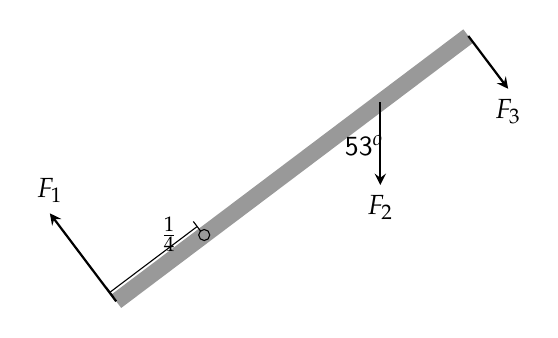
\begin{tikzpicture}[scale=0.7]
\draw[line width = 6pt,gray!80 ](0:0)--(37:8) coordinate(f3);
\draw [black] (37:2)circle (0.1cm);;
\draw[-stealth,thick](f3)--+(-53:1.2)node [below] {$F_3$};
\draw[-stealth,thick](0:0)--(127:2)node[above]{$F_1$};
\draw[|-|](127:0.2)--++(37:2);
\node [above] at (37:1.2){$\frac{1}{4}$};
\coordinate (f2) at (37:6);
\draw[-stealth, thick](f2)--++(-90:1.5)node[below]{$F_2$};
\node[below,xshift=-0.2cm,yshift=-0.3cm ] at (f2) {53$^o$}; 
\end{tikzpicture}\pilgan{
\item 0,8 N.m
\item 3,2 N.m 
\item 4,0 N.m
\item 7,4 N.m
\item [\lingkaran{E.}]8,0 N.m
} 
\hide{
\begin{align*}
\Sigma \tau &= \tau_1+\tau_2+\tau_3\\
\Sigma \tau &= 20.0,1+15.sin(53).0,2+12.0,3\\
\Sigma \tau &= 8N
\end{align*}
}
%----------------- nomor 2 ------
\item Berikut ini pernyataan tentang faktor-faktor gerak rotasi:
\pernyataan{
\item kecepatan sudut
\item letak sumbu rotasi
\item bentuk benda
\item massa benda
\item bentuk benda
\item massa benda
}
Faktor yang mempengaruhi besarnya momen inersia adalah . . . .
\pilgan{
\item 1,2,3, dan 4
\item 1,2, dan 3
\item 1,3, dan 4
\item [\lingkaran{D.}]2,3, dan 4
\item 2 dan 4
}
\hide{
Karena rumus inersia adalah $I=k.m.r^2$ maka: \begin{itemize}[topsep=0pt,itemsep=0pt]
\item $k$ konstanta tergantung bentuk benda
\item $m$ massa benda
\item $r$ letak sumbu rotasi (jari-jari pada benda lingkar)
\end{itemize}
}
%--------------------- nomor 3 ---------
\item Dua buah bola yang dianggap sebagai partikel dihubungkan dengan seutas tali kawat seperti gambar.
\begin{tikzpicture}[scale=0.7]
\draw [path picture={ \node at (path picture bounding box.center) {
\includegraphics[height=0.5cm]{bola.png}};},white] (0,1) circle (0.5);
\draw [path picture={ \node at (path picture bounding box.center) {
\includegraphics[height=0.5cm]{bola.png}};},white] (7,1) circle (0.5);
\draw[line width=0.1cm,gray!80](0.25,1)--node[below,scale=0.8,midway,black]{20cm}(2,1);
\draw[line width=0.1cm,gray!80](2,1)--node[below,scale=0.8,midway,black]{50cm}(6.8,1);
\draw[line width=-0.06cm,black](2,0)node[below]{A}--(2,2)node[above]{B};
\end{tikzpicture}

Bila massa bola P dan Q masing-masing 600 g dan 400 g, maka momen inersia sistem kedua bola terhadap poros AB adalah . . .
\pilgan{
\item 0,008 kg.m$^2$
\item 0,076 kg.m$^2$
\item [\lingkaran{C.}]0,124 kg.m$^2$
\item 0,170 kg.m$^2$
\item 0,760 kg.m$^2$
}
\hide{
Dari gambar tersebut bahwa $m_1$=0,6 kg, $m_2$ = 0,4 kg. Dan jarak terhadap sumbu rotasi $r_1$ = 0,2 m, $r_2$ = 0,5 m. Maka momen inersia sistem terhadap poros AB
\begin{align*}
\Sigma I &= m_1r_1^2+m_2r_2^2\\
\Sigma I &= 0,6.(0,2)^2+0,4.(0,5)^2\\
\Sigma I &= 0,124 \text{ kgm}^2
\end{align*}
}


%------------- nomor 4 -------------
\item Sebuah katrol dari benda pejal dengan tali yang dililitkan pada sisi luarnya ditampilkan seperti gambar. Gesekan katrol diabaikan. Jika momen inersia katrol $I=\beta$ dan tali ditarik dengan gaya tetap $F$, maka nila $F$ setara dengan . . . .

\begin{tikzpicture}[scale=1.5]
\draw[white](-2,0)--(2,0);
\draw[pattern=north east lines] (-0.5,0) rectangle (0.5,0.1);
\draw(0,-0.5) circle (0.45);
\draw[](-0.1,-1.1) rectangle (0.1,0);
\draw[-stealth](-0.45,-0.5)--+(0,-0.8) node[below,scale=0.9]{$F$};
\draw[-stealth](0,-0.5)--+(0.45,0);
\node at (0.2,-0.4)[scale=0.9]{R};
\end{tikzpicture}
\pilgan{
\item $F=\alpha.\beta.R$
\item $F=\alpha.\beta^2.R$
\item $F=\alpha.(\beta.R)^{-1}$
\item [\lingkaran{D.}]$F=\alpha.\beta.R^{-1}$
\item $F=(\alpha.\beta)^{-1}.R$
}
\hide{
\begin{align*}
\tau &= I.\alpha\\
F.R&= \beta. \alpha \\
F &= \alpha.\beta.R^{-1}
\end{align*}
}

%-------------- nomor 5 ----------
\item Katrol yang bermassa 10 kg dan jari-jarinya 25 cm digantungi massa benda 5 kg seperti pada gambar. Mula-mula massa benda diam kemudian dilepaskan maka perceptan sistem katrol adalah . . . ($I_{\text{katrol}} = \frac{1}{2} m.r^2)$

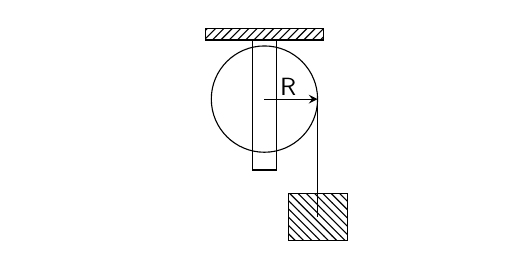
\begin{tikzpicture}[scale=1.5]
\draw[white](-2,0)--(2,0);
\draw[pattern=north east lines] (-0.5,0) rectangle (0.5,0.1);
\draw(0,-0.5) circle (0.45);
\draw[](-0.1,-1.1) rectangle (0.1,0);
\draw[-](0.45,-0.5)--+(0,-1.);
\draw [pattern=north west lines](0.2,-1.3)rectangle(0.7,-1.7);
\draw[-stealth](0,-0.5)--+(0.45,0);
\node at (0.2,-0.4)[scale=0.9]{R};
\end{tikzpicture}

\pilgan{
\item 1,0 m/s$^2$
\item 2,5 m/s$^2$
\item 3,3 m/s$^2$
\item [\lingkaran{D.}]5,0 m/s$^2$
\item 12,5 m/s$^2$
}
\hide{
\begin{align*}
a &= \frac{m.g}{m+k.m_{\text{katrol}}}=\frac{50}{5+\frac{1}{2}10}\\
a &= \frac{50}{10}=5 \text{ m/s}
\end{align*}

}



% ------------ nomor 6 ------------
\item Sebuah silinder penjal ($I=\frac{1}{2} m.r^2$) bergerak menggelinding tanpa tergelincir mendaki bidang miring kasar dengan kecepatan awal 10 m/s. Bidang miring itu mempunyai sudut elevasi $\alpha$ dengan sin $\alpha$ = 0,60. Jika percepatan gravitasi $g$ = 10 m/s$^2$ dan kecepatan benda berkurang menjadi 5 m/s, maka jarak yang ditempuh benda itu adalah . . . 

\pilgan{
\item 7,0 m
\item [\lingkaran{B.}]9,4 m
\item 12,0 m
\item 14,5 m
\item 17,0 m
}
\hide{
\begin{minipage}[T]{0.47\textwidth}
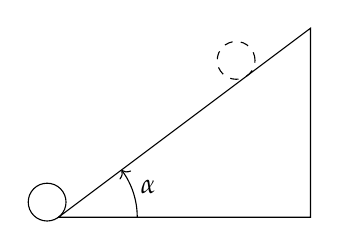
\begin{tikzpicture}[scale=0.8]
\draw (0,0) coordinate(o) --(4,0)coordinate(a)--(4,3)coordinate(b)--cycle;
\draw ($(0,0)+(127:0.3)$)circle(0.3cm);
\draw [dashed]($(3,2.25)+(127:0.3)$)circle(0.3cm);
\pic [draw, ->,"$\alpha$",angle radius=1cm,  angle eccentricity=1.2] {angle =a--o--b };
\end{tikzpicture}
\end{minipage}
\begin{minipage}[T]{0.47\textwidth}
Pada gambar di samping, menggunakan persamaan kekekalan energi mekanik rotasi pada keadaan di dasar dan saat kecepatan menjadi 5 m/s$^2$
\end{minipage}
\begin{align*}
EM_1 &= EM_2 \\
mgh+\frac{1}{2}m.v^2+\frac{1}{2}I.\omega^2 &=mgh_2 + \frac{1}{2}m.v_2^2+\frac{1}{2}I.\omega_2^2\\
mgh+\frac{1}{2}m.v_1^2(k+1)&=mgh_2+\frac{1}{2}m.v_2^2(k+1)\\
\coret{m}.g.0+\frac{1}{2}\coret{m}.10^2(\frac{1}{2}+1)&=\coret{m}.g.h_2 + \frac{1}{2}\coret{m}.5^2(\frac{1}{2}+1)\\
50(\frac{3}{2})-\frac{25}{2}(\frac{3}{2}) &=10.h_2\\
h_2&=\frac{225}{40}
\end{align*}
Maka besarnya jarak yang ditempuh adalah 
\begin{align*}
h&=R.sin \alpha\\
R&=\frac{h}{sin\alpha}\\
R&=\frac{\frac{225}{40}}{0,6}\\
R&=9,4 \text{ m}
\end{align*}
}
%---------------- nomor 7 ----------
\item Sebuah bendategar berada dalam kesetimbangan rotasi maka . . . .
\pilgan{
\item $\Sigma F_x=0$
\item $\Sigma F_y=0$
\item $\Sigma F_z=0$
\item $\Sigma \tau =0$
\item [\lingkaran{E.}]$\Sigma F=0$ dan $\Sigma \tau=0$
}
\hide{
Pada sistem seimbang syaratnya\\
 $\Sigma F=0$ dan $\tau = 0$
}
%---------------- nomor 8 ----------
\item Urutkan dari gambar-gambar di bawah ini yang termasuk kesetimbangan labil,stabil, atau netral!

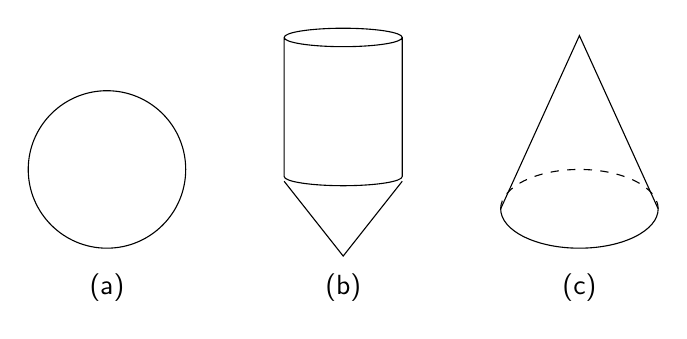
\begin{tikzpicture}
\draw (0,0) circle (1cm);
\node at (0,-1.5) {(a)};
\node (a) at (3,0.7) [cylinder, shape border rotate=90, draw, minimum height=20mm, minimum width=15mm]{};
\draw (2.25,-0.15)--(3,-1.1)--(3.75,-0.15);
\node at (3,-1.5) {(b)};
  \draw (5,-0.5) arc (180:360:1cm and 0.5cm) -- (6,1.7) -- cycle;
\node at (6,-1.5){(c)};
    \draw[dashed] (5,-0.5) arc (180:0:1cm and 0.5cm);
%    \shade[left color=blue!5!white,right color=blue!40!white,opacity=0.3] (-1,0) arc (180:360:1cm and 0.5cm) -- (0,3) -- cycle;
\end{tikzpicture}

\pilgan{ 
\item a,b,c
\item a,c,b
\item b,c,a
\item [\lingkaran{D.}]b,a,c
\item c,a,b
}
\hide{
stabil pada gambar (c)\\
labil(mudah jatuh) (b)\\
netral (a)
}

%-------------- nomor 9 ------------
\item Perhatikan gambar berikut! 

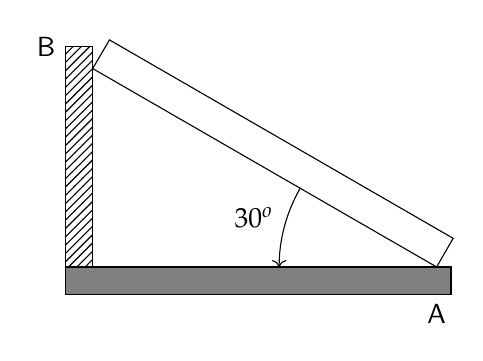
\begin{tikzpicture}[scale=0.7]
\draw(6.24,0)--(0,3.6)coordinate(b);
\draw(6.24,0)--($(6.24,0)+(60:0.6)$)--++(150:7.2)--(b);
\draw [pattern=north east lines] (-0.50,0) rectangle(0,4) ;
\node at (6.24,-0.5)[below]{A};
\node at (-0.5,4)[left] {B};
\coordinate (o) at (0,0);
\coordinate (t) at (6.24,0);
\coordinate (b) at (0,3.6);
    \pic [draw, ->,"$30^o$",angle radius=2cm,  angle eccentricity=1.2] {angle =b--t--o };

\draw [thin, fill =gray] (-0.5,0) rectangle (6.5,-0.5);
\end{tikzpicture}

Diketahui panjang batang AB 2,5 m dan berat 200 N serta batang bersandar pada dinding yang licin. Bila sistem batang dalam keadaan setimbang, maka koefisien gesekan batang dengan lantai adalah . . . 
\pilgan{
\item $\frac{1}{3}$
\item $\frac{1}{2}$
\item $\frac{1}{2}\sqrt{2}$
\item [\lingkaran{D.}] $\frac{1}{2}\sqrt{3}$
\item $\frac{1}{3}\sqrt{3}$
}

\hide{
Untuk tangga menyandar tanpa beban lain pada dinding licin, dan lantai kasar berlaku koefisien gaya gesek
\begin{align*}
\mu &=\frac{1}{2 tan \theta}\\
\mu &= \frac{1}{2.tan 30}\\
\mu &=\frac{1}{2.\sqrt{3}}\\
\mu &= \frac{1}{2} \sqrt{3}
\end{align*}
}

%------------- nomor 10 -------------
\item Perhatikan gambar bidang berikut!

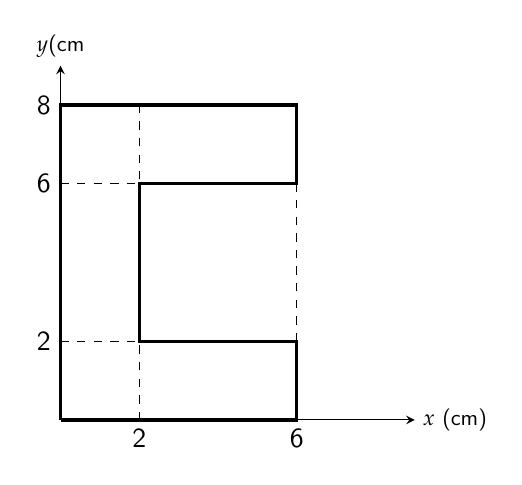
\begin{tikzpicture}[scale=0.5]
\draw[stealth-stealth](0,9) node [above, scale=0.8]{$y$(cm} -- (0,0) -- (9,0)node [right,scale=0.8]{$x$ (cm)};
\draw[very thick](0,0)--(6,0)--(6,2)--(2,2)--(2,6)--(6,6)--(6,8)--(0,8)--(0,0);
\foreach \x in {2,6}{\node at (\x,0) [below,scale=1] {\x};}
\foreach \y in {2,6,8}{\node at (0,\y)[left, scale=1]{\y};}
\draw[dashed](0,2)--(2,2)--(2,0)(6,2)--(6,6)(0,6)--(2,6)--(2,8);
\end{tikzpicture}

Koordinat titik berat dari benda tersebut adalah . . . .
\pilgan{
\item [\lingkaran{A.}](10/4 ; 16/4)
\item (12/4 ; 12/4)
\item (14/4 ; 14/4)
\item (16/4 ; 12/4)
\item (16/4 ; 10/4)
}
\hide{
Langkah pertama adalah membagi benda menjadi beberapa bagian

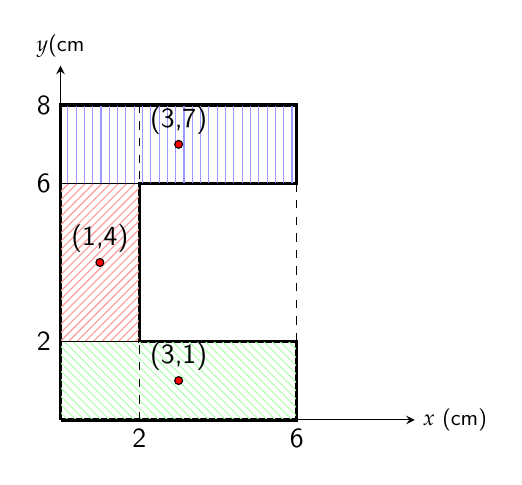
\begin{tikzpicture}[scale=0.5]
\draw[stealth-stealth](0,9) node [above, scale=0.8]{$y$(cm} -- (0,0) -- (9,0)node [right,scale=0.8]{$x$ (cm)};
\draw[very thick](0,0)--(6,0)--(6,2)--(2,2)--(2,6)--(6,6)--(6,8)--(0,8)--(0,0);
\draw[pattern=north west lines,pattern color=green!30](0,0) rectangle (6,2);
\draw[pattern color=red!40,pattern=north east lines](2,2) rectangle (0,6);
\draw[pattern=vertical lines,pattern color=blue!40](0,6) rectangle (6,8);
\foreach \x in {2,6}{\node at (\x,0) [below,scale=1] {\x};}
\foreach \y in {2,6,8}{\node at (0,\y)[left, scale=1]{\y};}
\draw[dashed](0,2)--(2,2)--(2,0)(6,2)--(6,6)(0,6)--(2,6)--(2,8);
\foreach \x/\y in{3/1,1/4,3/7}
{\draw[fill=red](\x,\y)circle(0.1cm);
\node at (\x,\y) [above]{(\x,\y)};
}
\end{tikzpicture}

\begin{align*}
x_{\text{cm}}&=\frac{x_1A_1+x_2A_2+x_3A_3}{A_1+A_2+A_3}\\
x_{\text{cm}}&=\frac{3.12+1.8+3.12}{12+8+12}\\
x_{\text{cm}}&=\frac{80}{32}=\frac{10}{4}
\end{align*}
\begin{align*}
y_{\text{cm}}&=\frac{y_1A_1+y_2A_2+y_3A_3}{A_1+A_2+A_3}\\
y_{\text{cm}}&=\frac{1.12+4.8+7.12}{12+8+12}\\
y_{\text{cm}}&=\frac{128}{32}=\frac{16}{4}
\end{align*}


}

%------------- nomor 11 -------------
\item Seutas kawat yang luas penampangnya 4 mm$^2$ ditarik oleh gaya 3,2 N, sehingga panjangnya bertambah 0,04 mm. Tegangan kawat tersebut adalah . . . .
\pilgan{
\item $ 8\times 10^6$ N/m$^2$
\item $ 7\times 10^6$ N/m$^2$
\item [\lingkaran{C.}]$ 8\times 10^5$ N/m$^2$
\item $ 8\times 10^4$ N/m$^2$
\item $ 5\times 10^4$ N/m$^2$
}
\hide{
\begin{align*}
\sigma &= \frac{F}{A}\\
\sigma &= \frac{3,2}{4\times 10^{-6}}\\
\sigma &= 8 \times 10^{5}
\end{align*}
}
%--------------- nomor 12 ------------
\item Seutas kawat baja yang panjangnya 1,0 m dengan luas penampang 2,0 mm$^2$ digunakan untuk mendukung beban 100 kg. Jika pertambahan panjang kawat baja 2,5 mm, maka regangan kawat tersebut adalah . . . .
\pilgan{
\item [\lingkaran{A.}]$2,5 \times 10^{-3}$
\item $2,5 \times 10^{-2}$
\item $2,5 \times 10^{-1}$
\item $4 \times 10^{2}$
\item $4 \times 10^{3}$
}
\hide{
\begin{align*}
e&=\frac{\Delta L}{L_o}\\
e&=\frac{2,5\times 10^{-3}}{1,0}\\
e&=2,5 \times 10^{-3}
\end{align*}

}


%---------------- nomor 13 ------------
\item Sebuah specimen baja berukuran 10 cm x 2 cm x 2 cm ditarik dengan gaya 5000 N bertambah panjang 5 mm. Modulus elastisitas Young bahan tersebut adalah . . . .
\pilgan{
\item $2,5 \times 10^9$ N/m$^2$ 
\item[\lingkaran{B.}] $2,5 \times 10^8$ N/m$^2$
\item $2,5 \times 10^6$ N/m$^2$
\item $4 \times 10^9$ N/m$^2$
\item $4 \times 10^8$ N/m$^2$
}
\hide{
Luas permukaan adalah 2cmx2cm = 4 cm$^2$=4$\times 10^{-4}$
Modulus elastisitas Young
\begin{align*}
Y &= \frac{F.L}{A.\Delta L}=\frac{5000.10\times 10^{-2}}{4\times 10^{-4}.5\times 10 ^{-3}}
Y&= 2,5 \times 10^8 \text{ N/m}^2
\end{align*}

}

%----------------- nomor 14 ----------- 
\item Kawat P dan Q terbuat dari bahan yangsama. Perbandingan antara diameter P dan Q adalah 2 : 3, sedangkan perbandingan antara panjang kawat P dan Q adalah 3 :4 . Dari data tersebut perbadingan antara konstanta gaya kawat P dan Q adalah . .  .
\pilgan{
\item 6 : 12
\item 8 : 9
\item 12 : 6
\item [\lingkaran{D.}]16 : 27
\item 27 : 16
} 
\hide{
karena kawat P dan Q adalah bahan sama, maka elastisitas/konstata young sama.
\begin{align*}
\frac{k_p}{k_q} &= \frac{\frac{F_p}{\Delta L_p}}{\frac{F_q}{\Delta L_q}} \\
\frac{k_p}{k_q} &= \frac{\frac{Y_p.A_p}{L_p}}{\frac{Y_q.A_q}{L_q}}\\
\frac{k_p}{k_q} &= \frac{\frac{2^2}{3}}{\frac{3^2}{4}}\\
\frac{k_p}{k_q} &= \frac{16}{27}
\end{align*}
}

%--------------- nomor 15 ----------
\item Sebuah pegas panjangnya 50 cm dengan konstanta pegas 200 N/m, dipotong menjadi dua bagian yang sama panjang. Potongan pegas tersebut ditarik dengan gaya 40 N akan bertambah panjang sebesar . . . 
\pilgan{
\item 5 cm
\item [\lingkaran{B.}]10 cm
\item 15 cm
\item 20 cm
\item 25 cm
}
\hide{
Saat benda dipotong menjadi dua, pegas yang baru (lebih pendek) mempunyai jenis elastisitas yang sama, namun besarnya konstanta pegas berubah
\begin{align*}
k&=\frac{F}{\Delta L}\\
\end{align*}
Sedangkan pada rumus elastisitas 
\begin{align*}
E&=\frac{FL}{A.\Delta L}\\
\end{align*}
Berarti diperoleh
\begin{align*}
k&=\frac{EA}{L}
\end{align*}
Karena panjang pegas menjadi separuh yakni $\frac{1}{2} L$ maka konstanta pegas menjadi $2k$
Pertmbahan panjang pegas jika ditarik dengan gaya 40N adalah . . .
\begin{align*}
\Delta x &= \frac{F}{k_{\text{pendek}}}=\frac{40}{2k}\\
\Delta x &= \frac{40}{2.200}=0,1 \text{ m}
\end{align*}
}

%------------- nomor 16 ----------
\item Grafik hubungan gaya (F) terhadap perubahan panjang dari percobaan elastisitas pegas di bawah ini. 

\begin{tikzpicture}
\draw[stealth-stealth](0,3)node [above]{$F$ (N)}--(0,0)--(3,0) node [right]{$\Delta x$(cm)};
\draw [dashed](0,2) node [left]{16}--(2,2)--(2,0)node [below]{4};
\draw (0,0) -- (2.5,2.5);
\end{tikzpicture}

Besarnya konstanta elastisitas pegas tersebut adalah . . . 
\pilgan{
\item 0,04 N/m
\item 0,4 N/m
\item 4 N/m
\item 40 N/m
\item [\lingkaran{E.}]400 N/m
}
\hide{
berdasarkan hukum hooke $F=k.\Delta x$ maka
\begin{align*}
F &= k. \Delta x \\
k &= \frac{F}{\Delta x}=\frac{16}{4\times 10^{-2}}=400 \text{ N/m}
\end{align*}
}

%------------ nomor 17 --------------
\item Sebuah benda bermassa 5 kg  menggantung pada sebuah pegas yang memiliki konstanta pegas sebesar 2.000 N/m. Bila $g$=10 m/s$^2$, pegas tersebut akan bertambah panjang sebesar . . . .
\pilgan{
\item 2,0 cm
\item [\lingkaran{B.}]2,5 cm
\item 4,0 cm
\item 5,0 cm
\item 6,5 cm
}
\hide{
\begin{align*}
\Delta x &= \frac {F}{k}\\
\Delta x &= \frac{m.g}{2000}=\frac{50}{2000}\\
\Delta x &= 2,5 \times 10^{-2} \text{ m} = 2,5 \text{ cm}
\end{align*}
}

%------------------ nomor 18 -----
\item Dua pegas identik dirangkai paralel dengan konstanta gaya pegas 100 N/m. Jika pada ujung susunan pegas diberi beban 10 N, maka pertambahan panjang masing-masing pegas adalah . . . .

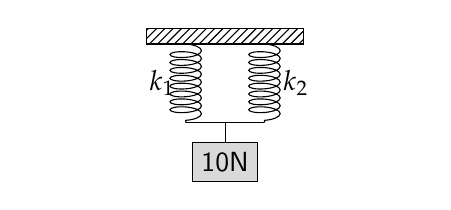
\begin{tikzpicture}
\draw[white](-2.5,0)--(2.5,0);
\draw[pattern=north east lines] (-1,0) rectangle (1,0.2);
\draw[decoration={aspect=0.3, segment length=1mm, amplitude=2mm,coil},decorate](-0.5,0)--+ (0,-1) coordinate(a);
\draw[decoration={aspect=0.3, segment length=1mm, amplitude=2mm,coil},decorate](0.5,0)--+(0,-1) coordinate(b);
\draw (a)--(b);
\draw[](0,-1)--+(0,-0.5) node(rect) [draw, fill=gray!30, minimum size=0.5cm]{10N};
\node at (-0.8,-0.5) {$k_1$};
\node at (0.9,-0.5) {$k_2$};
\end{tikzpicture}


\pilgan{
\item 1 cm
\item 2 cm
\item 3 cm
\item 4 cm
\item [\lingkaran{E.}]5 cm
}
\hide{
Jumlah konstanta kedua pegas yang paralel adalah 
\begin{align*}
k_{\text{total}} &= k_1 + k_2 = 200 \text{ N/m}
\end{align*}
Pertambahan panjang pegas total adalah
\begin{align*}
\Delta x &= \frac{F}{k_{\text{total}}}\\
\Delta x &= \frac{10}{200} = 5 \times 10^{-2} \text{ m}
\end{align*}
Karena pada susunan paralel $\Delta x_total = \Delta x_1 = \Delta x_2$ maka pertambahan panjang masing-masing pegas juga 5 cm
}

%--------------- nomor 19 ----------
\item Tiga pegas tersusun seperti gambar berikut.
 
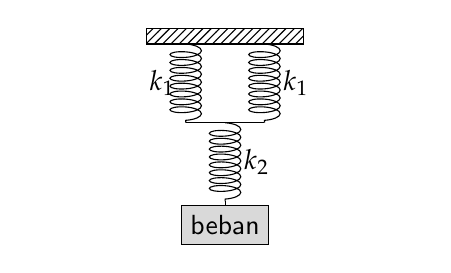
\begin{tikzpicture}
\draw[white](-2.5,0)--(2.5,0);
\draw[pattern=north east lines] (-1,0) rectangle (1,0.2);
\draw[decoration={aspect=0.3, segment length=1mm, amplitude=2mm,coil},decorate](-0.5,0)--+ (0,-1) coordinate(a);
\draw[decoration={aspect=0.3, segment length=1mm, amplitude=2mm,coil},decorate](0.5,0)--+(0,-1) coordinate(b);
\draw (a)--(b);
\draw[decoration={aspect=0.3, segment length=1mm, amplitude=2mm,coil},decorate](0,-1)--+(0,-1) coordinate(c);
\draw[](c)--+(0,-0.3) node(rect) [draw, fill=gray!30, minimum size=0.5cm]{beban};
\node at (-0.8,-0.5) {$k_1$};
\node at (0.9,-0.5) {$k_1$};
\node at (0.4,-1.5) {$k_2$};
\end{tikzpicture}

Jika tetapan pegas $k_1=k$ dan $k_2=4k$, maka nilai konstanta ($k'$) susunan pegas adalah . . . .
\pilgan{
\item $\frac{3}{4k}$
\item $\frac{3k}{4}$
\item[\lingkaran{C.}] $ \frac{4k}{3}$
\item $3k$
\item $4k$
}
\hide{
Paralel pegas atas (kiri dan kanan)
\begin{align*}
k_{\text{paralel}} &=k_1+k_1 = k+k=2k
\end{align*}
Hasil paralel diseri dengan $k_2$
\begin{align*}
\frac{1}{k_{\text{total}}} &= \frac{1}{k_2}+\frac{1}{k_{\text{paralel}}} \\
\frac{1}{k_{\text{total}}} &= \frac{1}{4k}+\frac{1}{2k} = \frac{1+2}{4k}=\frac{3}{4k}\\
k_{\text{total}} &= \frac{4k}{3}
\end{align*}
}

%-------------- nomor 20----------
\item Tiga buah pegas A,B, dan C yang identik dirangkai seperti gambar di bawah ini!.

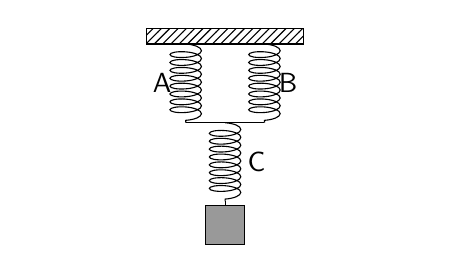
\begin{tikzpicture}
\draw[white](-2.5,0)--(2.5,0);
\draw[pattern=north east lines] (-1,0) rectangle (1,0.2);
\draw[decoration={aspect=0.3, segment length=1mm, amplitude=2mm,coil},decorate](-0.5,0)--+ (0,-1) coordinate(a);
\draw[decoration={aspect=0.3, segment length=1mm, amplitude=2mm,coil},decorate](0.5,0)--+(0,-1) coordinate(b);
\draw (a)--(b);
\draw[decoration={aspect=0.3, segment length=1mm, amplitude=2mm,coil},decorate](0,-1)--+(0,-1) coordinate(c);
\draw[](c)--+(0,-0.3) node(rect) [draw, fill=gray!80, minimum size=0.5cm]{};
\node at (-0.8,-0.5) {A};
\node at (0.8,-0.5) {B};
\node at (0.4,-1.5) {C};
\end{tikzpicture}

Jika ujunga bebas pegas C digantung beban 1,2 N maka sistem mengalami pertambahan panjang 0,6 cm, konstanta masing-masing pegas adalah . . . .
\pilgan{
\item 200 N/m
\item 240 N/m
\item [\lingkaran{C.}]300 N/m
\item 360 N/m
\item 400 N/m
}
\hide{
total konstanta pegas adalah . . .
\begin{align*}
\frac{1}{k_{\text{total}}} &= \frac{1}{k}+\frac{1}{2k}\\
\frac{1}{k_{\text{total}}} &= \frac{3}{2k}\\
k_{\text{total}} &= \frac{2k}{3}
\end{align*}
Menurut persamaan hukum hooke
\begin{align*}
F &= k.\Delta x \\
1,2 &= k_{\text{total}}.0,6\times 10^{-2}\\
k_{\text{total}} &=200 \text{ N/m}
\end{align*}
Sedangkan $k$ masing-masing pegas adalah
\begin{align*}
k_{\text{total}}&=\frac{2k}{3}\\
200 &=\frac{2k}{3}\\
k&=300 \text{  N/m}
\end{align*}
}
%A double line with ends are closed - manually created
%----------- nomor 21 -----------
\item Sebuah partikel bergerak sehingga menghasilkan persamaan posisi: $x=(3t^2 +5t - 2) $ m. Perpindahan benda dari detik ke 2 sampai dengan detik ke 5 adalah . . . 
\pilgan{
\item 75 m
\item [\lingkaran{B.}]78 m
\item 87 m
\item 57 m
\item 68 m
}
\hide{
perpindahan adalah $\Delta x = x_2-x_1$
\begin{align*}
x_1&=x(2)=3.2^2+5.2-2\\
x_1&=20
\end{align*}
\begin{align*}
x_2&=x(5)=3.5^2+5.5-2\\
x_2&=75+25-2=98
\end{align*}
\begin{align*}
\Delta x &= x_2-x_1=98-20=78
\end{align*}
}
%-------------- nomor 22 -------------
\item Vektor posisi yang dihasilkan oleh sebuah benda yang bergerak dalam bidang XY adalah $r=(t^3+2t^2-5t)\hat{\imath}+(t^2+2t+2)\hat{\jmath}$. Berapakah besar perpindahan yang dihasilkan benda dari awal sampai dengan detik ke-2?
\pilgan{
\item 4 m
\item 6 m
\item 8 m
\item [\lingkaran{D.}]10 m
\item 12 m
}
\hide{
Perpindahan adalah $\Delta r = r_2-r_1=r(2)-r(0)$
\begin{align*}
r_1&=r(0)=(t^3+2t^2-5t)\hat{\imath}+(t^2+2t+2)\hat{\jmath}\\
r_1&=2\hat{\jmath} \\
r_2&=r(2)=(2^3+2(2)^2-5.2)\hat{\imath}+(2^2+2.2+2)\hat{\jmath}\\
r_2&=6\hat{\imath}+10\hat{\jmath}
\end{align*}
Jadi perpindahannya adalah
\begin{align*}
\Delta r &= r_2-r_1=(6\hat{\imath}+10\hat{\jmath})-(2\hat{\jmath})\\
\Delta r &= 6\hat{\imath}+8\hat{\jmath}\\
\Delta r & = \sqrt{6^2+8^2}=10 \text{ m}
\end{align*}}
\end{enumerate}
\end{multicols*}
\end{document}

%--------------------- Selesai-------
